\begin{name}
	{\tenchude}
	{\tendethi}
	{\tentruong}
	{\thoigian}
\end{name}
\TN
\Opensolutionfile{ans}[ans/ans\currfilebase]
\begin{ex}%[2D1N1-1]
Hàm số nào dưới đây nghịch biến trên $\mathbb{R}$?
\choice
{\True $y=3-2x$}
{$y=x^2+2022$}
{$y=\dfrac{x-1}{x+2}$}
{$y=x^4-2x^2+2$}
\loigiai{
Ta có hàm số $y=3-2x$ có tập xác định $\mathscr{D}=\mathbb{R}$, hệ số $-2<0$ nên hàm số nghịch biến trên $\mathbb{R}$.
}
\end{ex}

\begin{ex}%[2D1N2-1]%[KNTT - Lớp 12 - Ôn tập cuối học kì 1 - Đề 6]%[Long]
Cho hàm số $y=f(x)$ có đạo hàm $y'=x(x+1)^2(x-1)^3$. Số điểm cực trị của hàm $f(x)$ là
\choice
{$1$}
{$3$}
{\True$2$}
{$0$}
\loigiai{
Ta có $y'=0\Leftrightarrow x(x+1)^2(x-1)^3=0$\\
$\Leftrightarrow\hoac{&x=0\\&x=-1\\&x=1}$ (nghiệm bội chẵn nên không là cực trị của $f(x)$.\\
Vậy số điểm cực trị của hàm $f(x)$ là $2$.
}
\end{ex}

\begin{ex}%[Mức độ N]%[2D1N2-1]
Hàm số nào dưới đây không có cực trị?
\choice{$y=\dfrac{x^2+1}{x}$}{\True $y=\dfrac{2x-2}{x+1}$}{$y=x^2-2x+1$}{$y=-x^3+x+1$}
\loigiai{Xét hàm số $y=\dfrac{2x-2}{x+1}\text{, } \forall x \ne-1$.\\ Ta có $y'=\dfrac{4}{(x+1)^2}>0\text{, } \forall x \ne -1$.\\
Vậy hàm số $y=\dfrac{2x-2}{x+1}$ không cực trị.}
\end{ex}

\begin{ex}%[2D1N5-4]
\immini{Cho hàm số có đồ thị như hình vẽ bên. Số giao điểm của đồ thị hàm số đã cho với trục hoành là
\choice
{$2$}
{$0$}
{\True $3$}
{$1$}}
{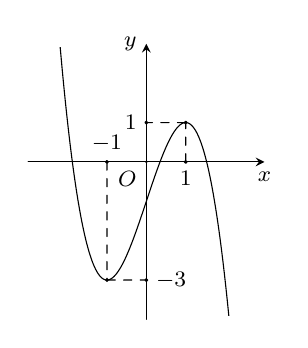
\begin{tikzpicture}[scale=0.5, font=\footnotesize, line join=round, line cap=round,>=stealth]
\def\a{-1} \def\b{0} \def\c{3} \def\d{-1}
\def\xmin{-3} \def\xmax{3}
\def\ymin{-4} \def\ymax{3}
\draw[->] (\xmin,0)--(\xmax,0) node [below]{$x$};
\draw[->] (0,\ymin)--(0,\ymax) node [left]{$y$};
\fill (0,0) circle (1.0pt) node [below left]{$O$};
\draw[dashed] (-1,0) circle (1.0pt) node [above]{$-1$}--(-1,-3)circle (1.0pt)--(0,-3) circle (1.0pt) node [right]{$-3$} (1,0)circle (1.0pt) node [below]{$1$}--(1,1)circle (1.0pt)--(0,1)circle (1.0pt) node [left]{$1$};
\clip (\xmin+0.1,\ymin+0.1) rectangle (\xmax-0.1,\ymax-0.1);
\draw[smooth,samples=300] plot(\x,{\a*(\x)^3+\b*(\x)^2+\c*(\x)+\d});
\end{tikzpicture}
}
\loigiai{
Đồ thị hàm số đã cho cắt trục hoành tại $3$ điểm.}
\end{ex}

\begin{ex}%[De-chuan-hoa-so-1]%[Mui Doan]%[2D1N3-1]
\immini{
Cho hàm số $f(x)$ liên tục trên $[-1;3]$ và có đồ thị như hình vẽ bên. Giá trị lớn nhất của hàm số trên $[-1;3]$ bằng
\choice
{$0$}
{$1$}
{$2$}
{\True $3$}
}{
\begin{tikzpicture}[scale=0.7, font=\footnotesize, line join=round, line cap=round,>=stealth]
\def\a{-1} \def\b{0} \def\c{2} % Hệ số
\def\xmin{-2} \def\xmax{4}
\def\ymin{-3} \def\ymax{4}
\draw[->] (\xmin,0)--(\xmax,0) node [below]{$x$};
\draw[->] (0,\ymin)--(0,\ymax) node [left]{$y$};
\node at (0,0) [below right]{$O$};
\clip (\xmin+0.1,\ymin+0.1) rectangle (\xmax-0.1,\ymax-0.1);
\draw[smooth,samples=300] plot[domain=-1:2](\x,{\a*(\x)^2+\b*(\x)+\c})--(3,3);
\draw[dashed] (-1,0)node[below]{$-1$}--(-1,1)--(0,1)node[right]{$1$}
(2,0)node[above]{$2$}--(2,-2)--(0,-2)node[left]{$-2$}
(3,0)node[below]{$3$}--(3,3)--(0,3)node[left]{$3$};
\fill (0,2) circle (1.0pt) node[above left]{$2$};
\end{tikzpicture}
}
\loigiai{
Từ đồ thị hàm số ta có $\max\limits_{x \in [-1;3]} f(x)=f(3)=3$.
}
\end{ex}

\begin{ex}%[2D1N4-1]
\immini[thm]{Cho hàm số $y=\dfrac{ax^2+bx+c}{mx+n}$ có đồ thị như hình bên. Tiệm cận xiên của đồ thị hàm số là
\choice
{$x=\dfrac{1}{2}$}
{$y=2x-1$}
{\True $y=\dfrac{1}{2}x+\dfrac{5}{4}$}
{$x=1$}
}
{
\begin{tikzpicture}[font=\footnotesize, line join=round, line cap=round,>=stealth,scale=1]
\draw[->] (-1.6,0)--(3.1,0) node[below left] {$x$};
\draw[->] (0,-.6)--(0,3.6) node[below left] {$y$};
\draw (0,0) node [below left] {$O$};
\draw (0.5,-.6)--(0.5,3.6);
\begin{scope}
\clip (-1.5,-.5) rectangle (3,3.5);
\draw[samples=200,domain=-1.5:0.49,smooth,variable=\x] plot (\x,{(1*((\x)^2)+2*(\x)+-1)/(2*(\x)+-1)});
\draw[samples=200,domain=0.51:2.5,smooth,variable=\x] plot (\x,{(1*((\x)^2)+2*(\x)+-1)/(2*(\x)+-1)});
\draw[samples=200,domain=-1.5:2.5,smooth,variable=\x] plot (\x,{.5*(\x)+1.25})node[sloped,rotate=30,below left]{$y=\tfrac{1}{2}x+\tfrac{5}{4}$};
\end{scope}
\end{tikzpicture}
}
\loigiai{
Ta thấy đồ thị hàm số có tiệm cận xiên là $y=\dfrac{1}{2}x+\dfrac{5}{4}$.
}
\end{ex}

\begin{ex}%[2D1N2-2]
Cho hàm số $y=f(x)$ có bảng biến thiên như hình vẽ
\begin{center}

\begin{tikzpicture}
\tkzTab[lgt=2,espcl=2.5,nocadre=false]
{$x$/1, $y'$/1, $y$/2.5}
{$-\infty$, $1$, $2$, $+\infty$}
{,+,0,-,0,+,}
{-/ $-\infty$, +/ $0$, -/ $-1$, +/ $+\infty$}
\end{tikzpicture}
\end{center}
Hàm số có giá trị cực tiểu bằng
\choice
{\True $-1$}
{$0$}
{$2$}
{$1$}
\loigiai{
Ta có điểm cực tiểu của hàm số là $x=2$ nên hàm số có giá trị cực tiểu bằng $y=-1$.
}
\end{ex}

\begin{ex}%[De-chuan-hoa-so-1]%[Hiệp Hà]%[2D1N1-2]
Cho hàm số $y=f(x)$ xác định trên $\mathbb{R}$ và có bảng biến thiên dưới đây. Khẳng định nào sau đây đúng?
\begin{center}

\begin{tikzpicture}
\tkzTabInit[lgt=1.2,espcl=2,deltacl=0.5]
{$x$/.7 ,$f'(x)$/.7,$f(x)$/2}
{$-\infty$,$-1$,$1$, $+\infty$}
\tkzTabLine{,+,0,-,0,+,}
\tkzTabVar{-/$-\infty$, +/$2$/,-/$-2$/,+/$+\infty$/}
\end{tikzpicture}
\end{center}
\choice
{Hàm số đồng biến trên khoảng $(-\infty;2)$}
{Hàm số đồng biến trên khoảng $(-1;+\infty)$}
{ Hàm số nghịch biến trên khoảng $(-2;2)$}
{\True Hàm số nghịch biến trên khoảng $(-1;1)$}
\loigiai{Theo bảng biến thiên, hàm số nghịch biến trên khoảng $(-1;1)$.}
\end{ex}

\begin{ex}%[2-D1B5-SO-17-2425]%[VN-MT-7, VM031]%[2D1N5-1]
\immini[thm]{Đường cong cho trong hình bên là đồ thị của hàm số nào trong các hàm số dưới đây?
\choice[2]
{$y=-x^3+2x-1$}
{$y=-x^3+3x+1$}
{$y=2x^3-6x+1$}
{\True $y=x^3-3x+1$}}
{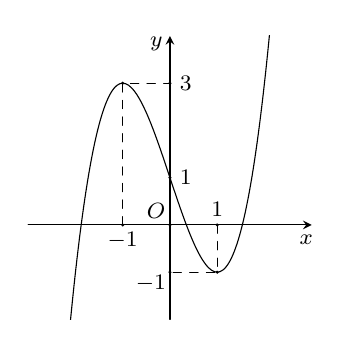
\begin{tikzpicture}[font=\footnotesize,line join=round, line cap=round, >=stealth,scale=0.6]
\def \xmin{-3}\def \xmax{3}\def \ymin{-2}\def \ymax{4}
\draw[->] (\xmin,0)--(\xmax,0) node[shift=(-110:0.2)] {$x$};
\draw[->] (0,\ymin)--(0,\ymax) node[shift=(-150:0.2)] {$y$};
\fill (0,0) circle(1pt) node[shift=(135:0.25)]{$O$}
(-1,0) circle(1pt) node[shift=(-90:0.2)]{$-1$}
(1,0) circle(1pt) node[shift=(90:0.2)]{$1$}
(0,-1) circle(1pt) node[shift=(-150:0.28)]{$-1$}
(0,1) circle(1pt) node[shift=(0:0.2)]{$1$}
(0,3) circle(1pt) node[shift=(0:0.2)]{$3$}
(-1,3) circle(1pt) (1,-1) circle(1pt);
\draw[dashed] (-1,0)|-(0,3) (1,0)|-(0,-1);
\clip (\xmin,\ymin) rectangle (\xmax,\ymax);
\draw[smooth,samples=100,domain=\xmin:\xmax] plot(\x,{(\x)^3-3*(\x)+1});
\end{tikzpicture}}
\loigiai{
Quan sát đồ thị, ta thấy
\begin{itemize}
\item Đây là đồ thị của hàm số $y=ax^3+bx^2+cx+d$ $ (a\ne 0)$ có $a > 0$.
\item Đồ thị hàm số có hai điểm cực trị $(-1;3)$ và $(1;-1)$.
\end{itemize}
Vậy đường cong trong hình vẽ là đồ thị hàm số $y=x^3-3x+1$.
}
\end{ex}

\begin{ex}%[2D1H1-5]
Sau khi phát hiện một bệnh dịch, các chuyên gia y tế ước tính số người nhiễm bệnh kể từ ngày xuất hiện bệnh nhân đầu tiên đến ngày thứ $t$ là $f(t)=45t^2-t^3$,  $t=0,1,2, \ldots, 25$. Nếu coi $f(t)$ là hàm số xác định trên đoạn $[0; 25]$ thì đạo hàm $f^{\prime}(t)$ được xem là tốc độ truyền bệnh (người/ngày) tại thời điểm $t$. Xác định khoảng thời gian mà tốc độ truyền bệnh giảm?
\choice
{$(0; 15)$}
{$(0; 10)$}
{$(15; 25)$}
{\True $(10; 25)$}
\loigiai{
Ta có $f^{\prime}(t)=90 t-3 t^2$ nên $f^{\prime \prime}(t)=90-6 t$.\\
Suy ra \[f^{\prime \prime}(t)=0 \Leftrightarrow t=15.\]
Bảng biến thiên như sau
\begin{center}

\begin{tikzpicture}[font=\normalsize]
%dòng khai báo
\tkzTabInit[lgt=1.2,espcl=3,deltacl=0.6]
{$t$/0.75, $f'' (t)$ /0.75,  $f'(t)$/2}
{$ 0 $, $ 15 $, $ 25$}
\tkzTabLine{,+,0,-,}
%dòng biến thiên
\tkzTabVar{-/$ $,+/$ $,-/$ $}
\end{tikzpicture}
\end{center}
Từ bảng biến thiên, trong khoảng thời gian $(15; 25)$ ngày thì tốc độ truyền bệnh giảm.
}
\end{ex}

\begin{ex}%[Dự án 2025 - đề cấu trúc mới, Hung Doan]%[2D1N5-1]
\immini{Đồ thị hình bên là của hàm số.
\choice
{$y=-x^3-3x^2+1$}
{$y=-x^3+3x^2+1$}
{$y=\dfrac{x^3}{3}-x^2+1$}
{\True $y=x^3-3x^2+1$}}{
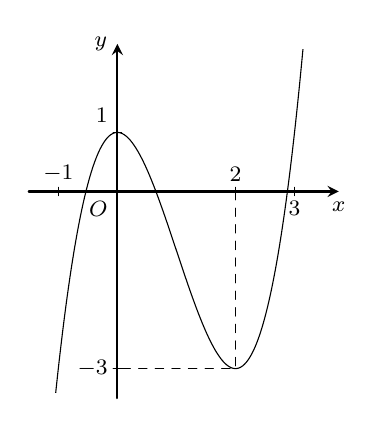
\begin{tikzpicture}[scale=0.75, font=\footnotesize, line join=round, line cap=round, >=stealth]
\def\xt{-1.5} \def\xp{3.75} \def\yt{2.5} \def\yd{-3.5}
\draw[->, line width=0.8pt](\xt, 0)--(\xp, 0) node[below]{$x$};
\draw[->, line width=0.8pt](0,\yd)--(0,\yt) node[left]{$y$};
\node at (0, 0) [below left]{$O$};
\clip(\xt+0.1,\yd+0.1) rectangle(\xp-0.1,\yt-0.1);
\draw[smooth,samples=300] plot(\x,{(\x)^3-3*(\x)^2+1});
\foreach \x in {-1,2}
\draw[shift ={ (\x,0)}]node[above]{$\x$} (0pt,2pt) --(0pt,-2pt);
\draw[shift ={ (3,0)}]node[below]{$3$} (0pt,2pt) --(0pt,-2pt);
\draw[shift ={ (0,-3)}]node[left]{$-3$} (2pt,0pt) --(-2pt,0pt);
\draw[shift ={ (0,1)}]node[above left]{$1$} (2pt,0pt) --(-2pt,0pt);
\draw[dashed] (2,0) -- (2,-3) -- (0,-3);
\end{tikzpicture}
}
\loigiai{
Dựa vào đồ thị ta thấy đây là đồ thị của hàm số bậc ba tổng quát có hệ số $a>0$ và đồ thị hàm số đi qua điểm $M(2;-3)$ nên đáp án cần chọn là $y=x^3-3x^2+1$.}
\end{ex}

\begin{ex}%[Dự án TL12New-4in1-NCT]%[2D1N4-1]
Cho hàm số có bảng biến thiên như sau:
\begin{center}

\begin{tikzpicture}[scale=1,line cap=round,line join=round,>=stealth]
\tkzTabInit[lgt=1.5,espcl=3]
{$x$/1,$y'$/.7,$y$/3}
{$-\infty$,$0$,$3$,$+\infty$}
\tkzTabLine{,-,d,-,z,+}
\tkzTabVar{+/$1$,-D+/$-\infty$/$2$,-/$-3$,+/$3$}
\end{tikzpicture}
\end{center}
Hỏi đồ thị của hàm số đã cho có tất cả bao nhiêu đường tiệm cận đứng và tiệm cận ngang?
\choice
{$4$}
{$1$}
{$2$}
{\True $3$}
\loigiai{
Ta có $\displaystyle \lim_{x\to 0^-}f(x)= - \infty$.
Do đó đồ thị hàm số có $1 $ đường tiệm cận đứng $x=0$, \\
$\displaystyle \lim_{x\to -\infty}f(x)= - 0$;$\displaystyle \lim_{x\to +\infty}f(x)= 3$ nên đường thẳng $y=0$; $y=3$ là tiệm cận ngang của đồ thị hàm số.
}
\end{ex}
\TNTF
\begin{ex}%[2D1V3-6]
Một hộ làm nghề dệt vải lụa tơ tằm sản xuất mỗi ngày được $ x $ mét vải lụa $ (1 \leq x \leq 18) $. Tổng chi phí sản xuất $ x $ mét vải lụa, tính bằng nghìn đồng, cho bởi hàm chi phí: $ C(x)=x^{3}-3 x^{2}-20 x+500 $. Giả sử hộ làm nghề dệt này bán hết sản phẩm mỗi ngày với giá $220$ nghìn đồng/mét. Gọi $ B(x) $ là số tiền bán được và $ L(x) $ là lợi nhuận thu được khi bán $ x $ mét vải lụa.
\choiceTF
{\True Biểu thức tính $ B(x) $ theo $ x $ là $ B(x)=220 x $ (nghìn đồng)}
{Biểu thức tính $ L(x) $ theo $ x $ là $ L(x)=-x^{3}+3 x^{2}+220 x-500 $ (nghìn đồng)}
{\True Hộ làm nghề dệt này cần sản xuất và bán ra mỗi ngày 10 mét vải lụa để thu được lợi nhuận tối đa}
{Lợi nhuận tối đa của hộ làm nghề dệt vải lụa tơ tằm có thể đạt được là 1000 nghìn đồng}
\loigiai{
\begin{itemchoice}
\itemch \textbf{Đúng}.\\
Số tiền thu được là: $ B(x)=220 x $ (nghìn đồng).
\itemch \textbf{Sai}.\\
Lợi nhuận thu được là: $ L(x)=B(x)-C(x)=-x^{3}+3 x^{2}+240 x-500 $ (nghìn đồng).
\itemch \textbf{Đúng}.\\
Hàm số $ L(x) $ xác định trên $ [1 ; 18] $.\\
Ta có $ L^{\prime}(x)=-3 x^{2}+6 x+240$, $L^{\prime}(x)=0 \Leftrightarrow x=10 $ hoặc $ x=-8 $ (loại).\\
Bảng biến thiên:
\begin{center}

\begin{tikzpicture}
\tkzTabInit
[lgt=3,espcl=5] % tùy chọn
{$x$/1, $L’(x)$/1, $L(x)$/2.5} % cột đầu tiên
{$1$, $10$, $18$} % hàng 1 cột 2
\tkzTabLine{,+,0,-,} % hàng 2 cột 2
\tkzTabVar{-/ $-258$, +/ $1200$ , -/ $-1040$} % hàng 3 cột 2
\end{tikzpicture}
\end{center}
Khi $ x=10 $ thì hàm số đạt giá trị lớn nhất là $1200$. Như vậy, hộ làm nghề dệt cần sản xuất và bán ra mỗi ngày $10$ mét vải lụa để thu được lợi nhuận tối đa.
\itemch \textbf{Sai}.\\
Lợi nhuận tối đa này là $1200$ nghìn đồng.
\end{itemchoice}
}
\end{ex}

\begin{ex}%[2D1H5-7]%[DA- EX-TF-TLN2024 - Phạm Quốc Toàn]
Cho hàm số $y=\dfrac{4x-3}{x-3}$ có đồ thị $\left(C \right)$. Xét tính đúng sai của các phát biểu sau.
\choiceTF
{\True Điểm $A \left(0; 1 \right)$ thuộc đồ thị $\left(C \right)$}
{Đồ thị $\left(C \right)$ không có điểm có tọa độ nguyên}
{\True Đồ thị $\left(C \right)$ có $6$ điểm có tọa độ nguyên}
{Biết đồ thị $\left(C \right)$ có hai điểm phân biệt $M$, $N$ và tổng khoảng cách từ $M$ hoặc $N$ tới hai tiệm cận là nhỏ nhất. Khi đó $MN$ có giá trị bằng $4 \sqrt{2}$}
\loigiai{
\begin{itemchoice}
\itemch {\bf Đúng}. Với $x =0 \Rightarrow y=1$. Vậy điểm $A \left(0; 1 \right)$ thuộc đồ thị $\left(C \right)$.
\itemch {\bf Sai}. Ta có $y= 4 + \dfrac{9}{x-3}$. \\
Để $y \in \mathbb{Z}$ thì $\dfrac{9}{x-3} \in \mathbb{Z} \Leftrightarrow \hoac{& x-3 = 1 \\ & x-3 = -1 \\ & x-3 =3 \\ & x-3 = -3 \\ & x-3 =9 \\ & x-3 = -9} \hoac{& x=4 \\ & x = 2 \\ & x = 6 \\ & x = 0 \\ & x = 12 \\ & x = -6.}$ \\
Vậy đồ thị $\left(C \right)$ vẫn có điểm có tọa độ nguyên.
\itemch {\bf Đúng}. Đồ thị $\left(C \right)$ có $6$ điểm có tọa độ nguyên.
\itemch {\bf Sai}. Giả sử $M=\left(m;\dfrac{4m-3}{m-3}\right)\in (C)$, với $m$ khác $3$.\\
Tiệm cận đứng là $x=3$, tiệm cận ngang là $y=4$.\\
Do đó tổng khoảng cách từ $M$ đến hai tiệm cận là \\
$\mathrm{d} =\left| m-3\right|+\left| \dfrac{4m-3}{m-3}-4\right| =\left| m-3\right|+\dfrac{9}{\left| m-3\right|} \ge 2 \cdot \sqrt{\left| m-3\right|\cdot \dfrac{9}{\left| m-3\right|}}=6$. \\
Dấu \rq\rq= \rq\rq xảy ra khi và chỉ khi $\left| m-3\right|=\dfrac{9}{\left| m-3\right|} \Leftrightarrow{(m-3)^2}=9$ \\
$\Leftrightarrow \hoac{&m-3=3 \\&m-3=-3} \Leftrightarrow \hoac{&m=6 \\&m=0}$.\\
Suy ra $\hoac{&M= \left(6;7 \right) \\&M= \left(0;1 \right)}$. \\
Một cách tương tự ta có các điểm $\hoac{&N= \left(6;7 \right) \\&N= \left(0;1 \right)}$.\\
Do $M$, $N$ phân biệt nên $MN=6 \sqrt{2}$.
\end{itemchoice}
}
\end{ex}

\begin{ex}%[2D1V3-6]
Một nhà sản xuất trung bình bán được $ 1\,000 $ laptop mỗi tuần với giá $14$ triệu đồng một chiếc. Một cuộc khảo sát thị trường chỉ ra rằng nếu cứ giảm giá bán $ 500 $ nghìn đồng, số lượng laptop bán ra sẽ tăng thêm khoảng $ 100 $ chiếc mỗi tuần. Biết rằng hàm chi phí hằng tuần là $C(x)=12\,000-3 x$ (triệu đồng), trong đó $x$ là số laptop bán ra trong tuần.\\
Xét tính đúng, sai của các phát biểu sau
\choiceTF[t]
{\True Hàm cầu là $p=-\dfrac{1}{200} x+19$, trong đó $ p $ (triệu đồng) là giá của mỗi laptop, $ x $ là số laptop bán ra}
{Để doanh thu đạt được là lớn nhất thì nên giảm giá bán laptop là $5$ triệu đồng cho một chiếc}
{Để công ty không bị lỗ vốn thì mỗi tuần cần bán được ít nhất $600$ chiếc laptop}
{\True Lợi nhuận lớn nhất mà công ty có thể đạt được là $12\,200$ (triệu đồng)}
\loigiai{
\begin{itemchoice}
\itemch	Gọi $ p $ (triệu đồng) là giá của mỗi laptop, $ x $ là số laptop bán ra. Khi đó ta cần xác định hàm cầu $p = p ( x )$.
\\
Theo giả thiết tốc độ thay đổi của $x$ tỉ lệ với tốc độ thay đổi của $p$ nên hàm số $p = p ( x )$ là hàm số bậc nhất. Do đó $p ( x )= ax + b\, ( a \neq 0)$.
\\
Theo đề bài, ta có $x_1=1\,000$ thì $p_1=14$ và $x_2=1\,100$ thì $p_2=13{,}5$.
\\
Khi đó đường thẳng có phương trình $p ( x )= ax + b$ đi qua hai điểm $(1\,000 ; 14)$ và $(1\,100 ; 13,5)$ nên ta có hệ phương trình
\[
\heva{&1\,000a+b=14 \\ &1\,100a+b=13{,}5}
\Leftrightarrow
\heva{&a=-\dfrac{1}{200} \\&b=19}
\]
Vậy, hàm cầu là $p=-\dfrac{1}{200} x+19$.
\itemch	Vì $p=-\dfrac{1}{200} x+19$ nên $x=-200 p+3\,800$.
\\
Khi đó tổng doanh thu từ tiền bán laptop là
\[
R(p)=x \cdot p=(-200 p+3\,800) \cdot p=-200 p^2+3\,800 p .
\]
Bài toán trở thành tìm $p$ để $R(p)$ đạt giá trị lớn nhất.
\\
Ta có
\[
R'(p)=-400 p+3800; \quad R'(p)=0 \Leftrightarrow p=9{,}5.
\]
Bảng biến thiên
\begin{center}

\begin{tikzpicture}[font=\footnotesize,thick,>=stealth]
\tikzset{double style/.append style={double distance=1.5pt}}
\tkzTabInit[nocadre=false,
lgt=1.2,
espcl=3.5,
deltacl=0.6,
lw=.75pt,color]
{$p$ /1.2, $R'(p)$ /1, $R(p)$ /2.5}
{$0$,$9{,}5$,$+\infty$}
\tkzTabLine{ ,+,$0$,-, }
\tkzTabVar{-/$0$,+/$18\,050$,-/$-\infty$}
\end{tikzpicture}
\end{center}
Dựa vào bảng biến thiên ta thấy công ty giảm giá $14-9{,}5=4{,}5$ triệu đồng cho người mua thì doanh thu của công ty sẽ lớn nhất.
\itemch	Doanh thu từ bán $x$ laptop là $R(x)=x \cdot p(x)=x\left(-\dfrac{1}{200} x+19\right)=-\dfrac{1}{200} x^2+19 x$.
\\
Khi đó tổng lợi nhuận từ bán $x$ laptop là
\begin{align*}
P ( x )&= R ( x )- C ( x ) \\
& =-\dfrac{1}{200} x^2+19 x-(12\,000-3 x) \\
& =-\dfrac{1}{200} x^2+22 x-12\,000
\end{align*}
Để công ty không bị lỗ vốn thì
\begin{eqnarray*}
P(x) \ge 0 &\Leftrightarrow& -200\sqrt{61}+2200\le \:x\le \:200\sqrt{61}+2200 \\
&\approx& 638 \le \:x\le \:3762.
\end{eqnarray*}
\itemch	Lợi nhuận từ bán $x$ laptop là $R(x)=-\dfrac{1}{200} x^2+22 x-12\,000$.\\
Bài toán trở thành tìm $x$ để $P ( x )$ lớn nhất.
\\
Ta có
\[
P'(x)=-\dfrac{1}{100} x+22; \quad P'(x)=0 \Leftrightarrow-\dfrac{1}{100} x+22=0 \Leftrightarrow x=2\,200.
\]
Bảng biến thiên
\begin{center}

\begin{tikzpicture}[font=\footnotesize,thick,>=stealth]
\tikzset{double style/.append style={double distance=1.5pt}}
\tkzTabInit[nocadre=false,
lgt=1.2,
espcl=3.5,
deltacl=0.6,
lw=.75pt,color]
{$x$ /1.2, $R'(x)$ /1, $R(x)$ /2.5}
{$0$,$2\,200$,$+\infty$}
\tkzTabLine{ ,+,$0$,-, }
\tkzTabVar{-/$0$,+/$12\,200$,-/$+\infty$}
\end{tikzpicture}
\end{center}
Dựa vào bảng biến thiên ta thấy số laptop bán ra trong 1 tuần là $ 2\,200 $ chiếc thì lợi nhuận đạt giá trị lớn nhất là $12\,000$ (triệu đồng).
\end{itemchoice}
}
\end{ex}

\begin{ex}%[2D1H5-4]
Cho hàm số $y=\dfrac{2x+1}{x-1}$. Xét tính đúng, sai trong các khẳng định sau
\choiceTF
{Đồ thị hàm số $y=\dfrac{2x+1}{x-1}$ cắt trục $Ox$ tại điểm có hoành độ bằng $1$}
{\True Đường thẳng $y=x-2$ cắt đồ thị hàm số $y=\dfrac{2x+1}{x-1}$ tại hai điểm phân biệt $A,B$ có hoành độ lần lượt $x_A,x_B$ và $x_A+x_B=5$}
{Không có giá trị nào của $m$ để đường thẳng $y=m$ và đồ thị hàm số $y = \dfrac{2x + 1}{x - 1}$ có điểm chung}
{\True Có $17$ giá trị nguyên của $m$ thuộc đoạn $\left[-14; 15\right]$ sao cho đường thẳng $y = mx + 3$ cắt đồ thị của hàm số $y = \dfrac{2x + 1}{x - 1}$ tại hai điểm phân biệt}

\loigiai{
\begin{itemchoice}
\itemch
$Ox\colon y=0$.\\
Phương trình hoành độ giao điểm giữa $y=\dfrac{2x+1}{x-1}$ và $y=0$ là
\[\dfrac{2x+1}{x-1}=0\Leftrightarrow x=-\dfrac{1}{2}.\]
Do đó đồ thị hàm số $y=\dfrac{2x+1}{x-1}$ cắt trục $Ox$ tại điểm có hoành độ bằng $-\dfrac{1}{2}.$
\itemch
Phương trình hoành độ giao điểm giữa $y=\dfrac{2x+1}{x-1}$ và $y=x-2$ là \[x-2=\dfrac{2x+1}{x-1} \Leftrightarrow x^2-3x+2=2x+1 \Leftrightarrow x^2-5x+1=0.\]
Do đó $x_A+x_B=5$.
\itemch
Phương trình hoành độ giao điểm giữa $y=\dfrac{2x+1}{x-1}$ và $y=m$ là
\[y=\dfrac{2x+1}{x-1}=m\Leftrightarrow (2-m)x=-m-1.\quad(*)\]
$(*)$ có nghiệm khi $2-m\ne 0\Leftrightarrow m\ne 2.$\\
Vậy $m\ne 2$ đường thẳng $y=m$ và đồ thị hàm số $y = \dfrac{2x + 1}{x - 1}$ có điểm chung
\itemch
Phương trình hoành độ giao điểm $mx + 3 = \dfrac{2x + 1}{x - 1} \Leftrightarrow mx^2 + x(1 - m) - 4 = 0$ \quad (*).
\begin{itemize}
\item Với $m = 0$ thì phương trình ($*$) có một nghiệm $x = 4$.
\item Với $m \neq 0$, xét biệt thức $\Delta = m^2 + 14m + 1$.
\end{itemize}
Đồ thị của hai hàm số cắt nhau tại hai điểm phân biệt nên \[\Delta > 0 \Leftrightarrow m^2 + 14m + 1 > 0 \Leftrightarrow \hoac{&m > - 7 + 4\sqrt{3}\approx -0{,}08\\&m< - 7 - 4\sqrt{3}\approx -13{,}9.}\]
$\Rightarrow m \in\{-14,0,1,2,3,\cdots,15\}$
Vậy có $17$ giá trị nguyên của $m \in [-14; 15]$ thỏa mãn yêu cầu bài toán.
\end{itemchoice}
}
\end{ex}
\TNSA
\begin{ex}%[SGK 12 - Cùng Khám Phá, Mức độ 4]%[BG12-4IN1, Nguyễn Khánh Trọng]%[2D1C3-6]
\immini{Một thùng chứa nhiên liệu gồm phần ở giữa là một hình trụ có chiều dài $h$ mét $(h>0)$ và hai đầu là các nửa hình cầu bán kính $r$ $(r>0)$ (\textit{Hình 1.11}). Biết rằng thể tích của thùng chứa là $144\,000 \pi$ m$^3$. Để sơn mặt ngoài của phần hình cầu cần $20\,000$ đồng cho $1$ m$^2$, còn sơn mặt ngoài cho phần hình trụ cần $10\,000$ đồng cho $1$ m$^2$. Xác định $r$ để chi phí cho việc sơn diện tích mặt ngoài thùng chứa (bao gồm diện tích xung quanh hình trụ và diện tích hai nửa hình cầu) là nhỏ nhất, biết rằng bán kính $r$ không được vượt quá $50$ m.
\shortans{$30$}
}{

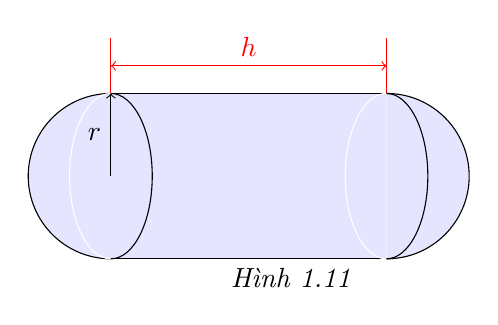
\begin{tikzpicture}[scale=.7]
\draw[white,fill=blue!10] (0,0) rectangle (5,3);
\draw(0,0)--(5,0);
\draw(0,3)--(5,3);
\draw[red](0,3)--(0,4);
\draw[red](5,3)--(5,4);
\draw[fill=blue!10] (5,3) arc(90:-90:1.5);
\draw[fill=blue!10] (0,0) arc(-90:-270:1.5);
\draw[white] (0,3) arc (90:270:0.75 and 1.5);
\draw (0,0) arc (-90:90:0.75 and 1.5);
\draw[white] (5,3) arc (90:270:0.75 and 1.5);
\draw (5,0) arc (-90:90:0.75 and 1.5);
\draw[red,<->] (0,3.5)--(5,3.5) node[midway,above]{$h$};
\draw[->] (0,1.5)--(0,3) node[midway,left]{$r$};
\draw (2,0) node[below right]{\textit{Hình 1.11}};
\end{tikzpicture}
}
\loigiai{
Ta có thể tích của thùng chứa nhiên liệu là $V=\pi \cdot r^2 \cdot h + \dfrac{4}{3} \pi \cdot r^3 = 144\, 000 \pi$ \\
Suy ra $h=\dfrac{(144\,000-\dfrac{4}{3} \cdot r^3)}{r^2}$ \\
Khi đó chi phí sơn diện tích mặt ngoài thùng chứa là
\[2 \pi \cdot r \cdot \dfrac{(144\,000-\dfrac{4}{3} \cdot r^3)}{r^2} \cdot 10^4 + 4 \pi \cdot r^2 \cdot 2 \cdot 10^4 =2 \pi \cdot 10^4 \left( \dfrac{144\,000}{r} + \dfrac{8}{3} r^2 \right). \]
Xét hàm số $f(r)=\dfrac{144\,000}{r} + \dfrac{8}{3} r^2$ với $r \in (0;50]$.\\
Ta có $f^{\prime}(r)=-\dfrac{144\,000}{r^2} + \dfrac{16}{3} r=\dfrac{16r^3-432\,000}{3r^2}$ và $f^{\prime}(r)=0 \Leftrightarrow r=30$ m.\\
Bảng biến thiên\\
\begin{center}

\begin{tikzpicture}
\tkzTabInit[nocadre=false,lgt=1.2,espcl=3.5,deltacl=0.6]
{$r$/1,$f'(r)$/1,$f(r)$/3}
{$0$,	$30$,	$50$}
\tkzTabLine{,	-,	$0$,	+}
\tkzTabVar{+/$+\infty$,	-/$7200$,	+/$9546{,}7$}
\end{tikzpicture}
\end{center}
Vậy với $r=30$ m thì chi phí cho việc sơn diện tích mặt ngoài của thùng chứa là nhỏ nhất.
}
\end{ex}

\begin{ex}%[2D1V3-6]
Độ giảm huyết áp của một bệnh nhân được cho bởi công thức $G(x)=0{,}025x^{2} (30-x)$, trong đó $x$ là liều lượng thuốc được tiêm cho bệnh nhân ($x$ được tính bằng mi-li-gam). Bác sĩ cần phải tiêm liều lượng thuốc ít nhất để huyết áp giảm?
\shortans{$20$}
\loigiai{
Ta có: $G(x)=0{,}75x^{2} -0{,}025x^{3} \Rightarrow G'(x)=1{,}5x-0{,}075x^{2} =0 \Rightarrow \hoac{&x=0\\&x=20.}$\\
Bảng biến thiên
\begin{center}

\begin{tikzpicture}
\tkzTabInit[nocadre=true,lgt=1.5,espcl=3,deltacl=0.8]
{$x$/.7 ,$G'(x)$/.7,$G(x)$/2}
{$0$ ,  $20$ , $+\infty$}
\tkzTabLine{, + , $0$ , -  }
\tkzTabVar{-/$ $ , +/$100$ , -/$ $}
\end{tikzpicture}
\end{center}
Huyết áp bệnh nhân giảm  khi liều lượng thuốc cần tiêm ít nhất là $20$ miligam.
}
\end{ex}

\begin{ex}%[Trần Công Duy]%[MathTex_TN THPT 2026]%[2D1V4-3]
Nồng độ thuốc trong máu của một bệnh nhân sau khi tiêm $t$ giây là $P(t)\left(\dfrac{\text{mg}}{\text{ml}}\right)$. Với $P(t)$ cho bởi công thức $P(t)=\sqrt{0{,}09 t^2+0{,}018 t+0{,}05}-0{,}3 t$. Nồng độ thuốc tồn dư, tức nồng độ thuốc vẫn còn trong cơ thể bệnh nhân trong dài hạn khi tiêm là bao nhiêu?
\par
\shortans[0]{0{,}03}
\loigiai{
Ta có
$\begin{aligned}[t]
\lim\limits _{t \rightarrow+\infty} P(t)
&=\lim\limits _{t \rightarrow+\infty}\left(\sqrt{0{,}09 t^2+0{,}018 t+0{,}05}-0{,}3 t\right)\\
&=\lim\limits _{t \rightarrow+\infty} \dfrac{0{,}09 t^2+0{,}018 t+0{,}05-(0{,}3 t)^2}{\sqrt{0{,}09 t^2+0{,}018 t+0{,}05}+0{,}3 t} \\
&=\lim\limits _{t \rightarrow+\infty} \dfrac{0{,}018 t+0{,}05}{\sqrt{0{,}09 t^2+0{,}018 t+0{,}05}+0{,}3 t}\\
&=\lim\limits _{t \rightarrow+\infty} \dfrac{t\left(0{,}018+\dfrac{0{,}05}{t}\right)}{t\left(\sqrt{0{,}09+\dfrac{0{,}018}{t}+\dfrac{0{,}05}{t^2}}+0{,}3\right)}\\
&=\lim\limits _{t \rightarrow+\infty} \dfrac{0{,}018+\dfrac{0{,}05}{t}}{\sqrt{0{,}09+\dfrac{0{,}018}{t}+\dfrac{0{,}05}{t^2}}+0{,}3}
=\dfrac{0{,}018}{\sqrt{0{,}09}+0{,}3}=0{,}03.
\end{aligned}$\\
Vậy nồng độ thuốc tồn dư trong cơ thể bệnh nhân là $0{,}03~\left(\dfrac{\text{mg}}{\text{ml}}\right)$.
}
\end{ex}

\begin{ex}%[2D1V3-2]
Tìm giá trị nhỏ nhất của hàm số $ f(x) = \dfrac{2}{x^2} - \dfrac{1}{2x-2}$ trên khoảng $(0;1)$. (kết quả làm tròn đến hàng phần chục).
\shortans{5{,}5}
\loigiai
{
Hàm số xác định và liên tục trên $(0;1)$ và có $f'(x)=-\dfrac{4}{{x^3}}+\dfrac{1}{2{{(x-1)}^2}}$.\\
Giải phương trình $f'(x)=0 \Leftrightarrow  {x^3}-8{x^2}+16x-8=0 \Leftrightarrow  (x-2)({x^2}-6x+4)=0$\\
$\Rightarrow  x=3-\sqrt {5}$ (do $ x\in (0;1)$).\\
Bảng biến thiên
\begin{center}

\begin{tikzpicture}
\tkzTabInit[nocadre=false,lgt=1.2,espcl=3,deltacl=0.6]
{$x$/0.7,$y'$/0.7,$y$/2.5}
{$0$,$3-\sqrt{5}$,$1$}
\tkzTabLine{,-,0,+,}
\tkzTabVar{+/$+\infty$,-/$\dfrac{11+5\sqrt{5}}{4}$,+/$+\infty$}
\end{tikzpicture}
\end{center}
Từ bảng biến thiên ta có $\min\limits_{(0;1)}f(x)=\dfrac{11+5\sqrt {5}}{4}\approx 5{,}5$.
}
\end{ex}

\begin{ex}%[2-D1B3-SO-8-2425]%[VN-MT-7, Nguyễn Hồng Thạch]%[2D1C4-3]
Người ta thống kê được chi phí sửa chữa, vận hành máy móc trong một năm của xưởng sản xuất được tính bởi công thức $f(x)=\dfrac{2\,000x-1\,500}{35x+5}$ (triệu đồng). Biết $x$ là số năm kể từ lúc máy móc vận hành lần đầu tiên, số năm càng nhiều thì chi phí càng cao. Khi số năm $x$ đủ lớn thì chi phí vận hành máy móc trong một năm gần với số nào? (làm tròn kết quả đến hàng phần chục).

\shortans{57{,}1}

\loigiai{
Ta có $\lim\limits_{x\to +\infty} f(x)=\lim\limits_{x\to+\infty}\dfrac{2\,000x-1\,500}{35x+5}=\dfrac{400}{7}$.\\
Do đó đồ thị hàm số $y=f(x)$ nhận đường thẳng $y=\dfrac{400}{7}$ làm tiệm cận ngang, tức là khi số năm $x$ càng lớn thì chi phí vận hành máy móc trong một năm càng tiến gần đến $\dfrac{400}{7}\approx 57{,}1$ (triệu đồng).
}
\end{ex}

\begin{ex}%[De-chuan-hoa-so-1]%[Lâm Chính]%[2D1H1-3]
Hỏi có bao nhiêu số nguyên $m$ để hàm số $y=\left(m^2-1\right)x^3+(m-1)x^2-x+4$ nghịch biến trên khoảng $(-\infty;+\infty)$?
\shortans[]{$2$}
\loigiai{
Tập xác định $\mathscr{D}=\mathbb{R}$.\\
Ta có $y'=3\left(m^2-1\right)x^2+2(m-1)x-1$.\\
Hàm số đã cho nghịch biến trên $\mathbb{R} \Leftrightarrow y'\le 0,\forall x\in\mathbb{R} \quad(*)$.\\
Với $m=-1$ thì ta có $y'=-4x-1$, không thoả mãn.\\
Với $m=1$ thì ta có $y'=-1<0, \forall x\in \mathbb{R}$, thoả mãn.\\
Với $m\ne \pm 1$, ta có $3\left(m^2-1\right)\ne 0$ nên\\
$(*)\Leftrightarrow \heva{&3\left(m^2-1\right)<0 \\ &\Delta'\le 0}\Leftrightarrow \heva{&m^2-1<0 \\ &(m-1)^2+3(m^2-1)\le 0} \Leftrightarrow \heva{&-1<m<1 \\ &-\dfrac{1}{2}\le m\le 1}\Leftrightarrow -\dfrac{1}{2}\le m<1$.\\
Vậy có $2$ giá trị nguyên $m$ thoả mãn bài toán là $m=0 \vee m = 1$.
}
\end{ex}
\Closesolutionfile{ans}
